\autobookmark
\begin{frame}[t]{Sample points can be distributed in a cluster}
  \begin{columns}[T]

    \begin{column}{.5\textwidth}
      \myonly{1}{
\includegraphics[width=0.5\paperwidth]{graphics/load_balancing_MPI_0.pdf}}
      \myonly{2}{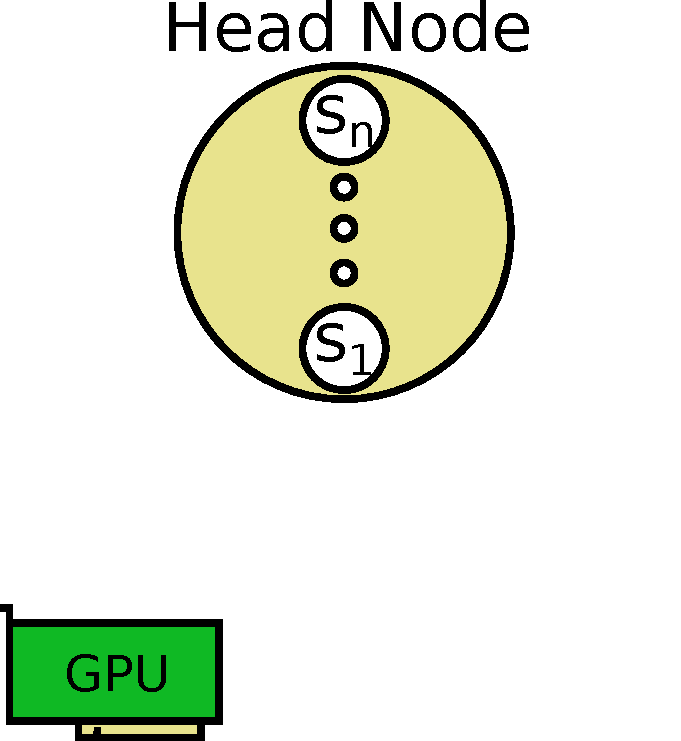
\includegraphics[width=0.5\paperwidth]{graphics/load_balancing_MPI_1.pdf}}
      \myonly{3}{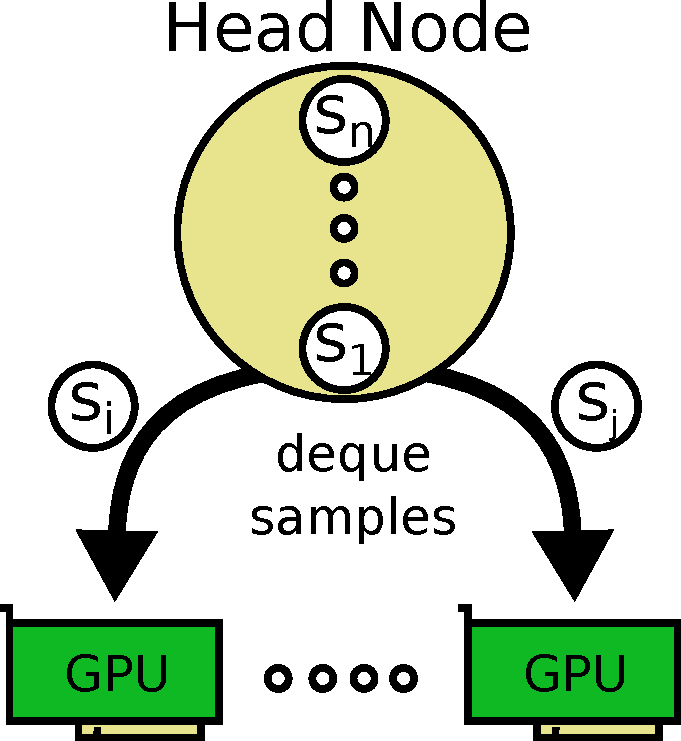
\includegraphics[width=0.5\paperwidth]{graphics/load_balancing_MPI_2.pdf}}
      \myonly{4-}{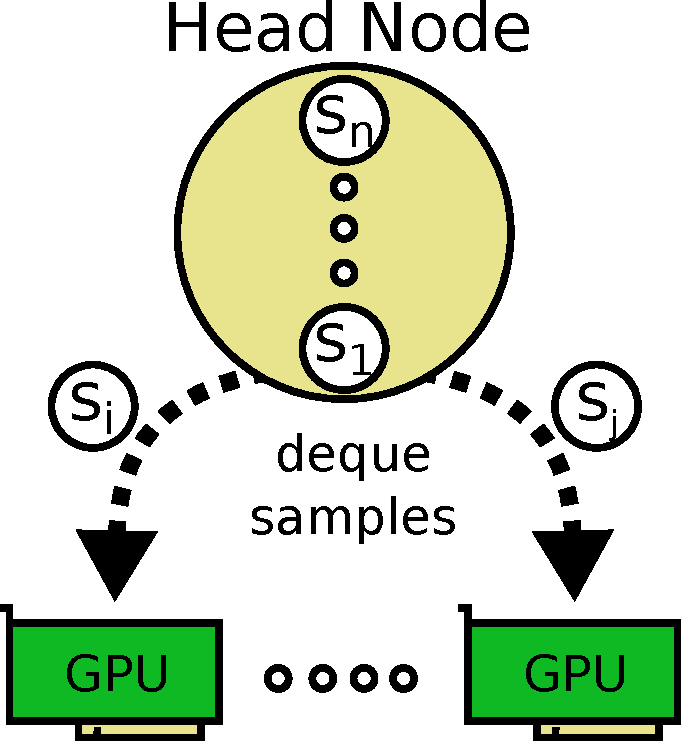
\includegraphics[width=0.5\paperwidth]{graphics/load_balancing_MPI_3.pdf}}
    \end{column}

    \begin{column}{.5\textwidth}
      \begin{itemize}
          \myuncover{1}{5}{
            \item Until now: simulation of a single sample point on a single GPU
          }
          \myuncover{2}{5}{
            \item All sample points are independent: let's use a cluster for that
            \item Each GPU has all the necessary data
          }
          \myuncover{3}{5}{
            \item MPI is used as communication framework
            \item Head node assigns work to the GPU
          }
          \myuncover{4}{5}{
            \item Add more GPUs as needed
          }
          \myuncover{5}{5}{
            \item Load balancing, even when some sample points take longer than others
          }
      \end{itemize}
    \end{column}

  \end{columns}
\end{frame}

%\begin{frame}{Predefined colours}
%  The template defines a set of colours according to the CD guidelines:\par
%  \begin{itemize}
%      \begin{minipage}[t]{0.5\linewidth}
%      \item \textcolor{hzdr-blue}{Helmholtz Blue}    
%      \item \textcolor{hzdr-orange}{Rossendorf Orange}  
%      \item \textcolor{hzdr-darkblue}{Helmholtz Dark Blue}
%      \item \textcolor{hzdr-gray1}{Gray1}   
%      \item \textcolor{hzdr-gray2}{Gray2}   
%      \item \textcolor{hzdr-gray3}{Gray3}   
%      \item \textcolor{hzdr-struct}{Structure of Matter}  
%      \end{minipage}%
%      \begin{minipage}[t]{0.5\linewidth}
%      \item \textcolor{hzdr-health}{Health}  
%      \item \textcolor{hzdr-energy}{Energy}  
%      \item \textcolor{hzdr-earth}{Earth and Environment}   
%      \item \textcolor{hzdr-keytec}{Key Technologies}  
%      \item \textcolor{hzdr-aero}{Aeronautics, Space and Transport}
%      \end{minipage}
%  \end{itemize}
%\end{frame}

